\documentclass{beamer}
\usepackage{graphicx}
\usepackage{epstopdf}
\usepackage{multirow}
\usepackage{booktabs}
\usepackage{xcolor}

\usetheme[
        %url={nano.uoft.ca},
        %numbering={false},
        menuwidth={0.3\paperwidth}
        ]{uoft}

\setbeamercovered{transparent=20}
\graphicspath{
{/home/schuberm/Dropbox/git/plots.nogit/images/}
{/Users/mullspace/Dropbox/git/plots.nogit/images/}
{/home/schuberm/Dropbox/UofT/uoft_thesis/images/}
{/Users/mullspace/Dropbox/UofT/uoft_thesis/images/}
{/home/mullspace/Dropbox/git/plots.nogit/images/}
{/home/mullspace/Dropbox/UofT/uoft_thesis/images/}}

%--------------------------------------------------------------------------
%DEFINE COMMANDS
%--------------------------------------------------------------------------
\newcommand{\EXP}[1]{\exp\mspace{-5.0mu}\left[#1\right]\mspace{-3.0mu}}

\newcommand{\SUM}[2]{\ifthenelse{\equal{#1}{0}}{\sum_{
\alpha_{#2},b_{#2},l_{#2}}^{3,4L,N}} {\ifthenelse{\equal{#1}{1}}{\sum_{
\alpha_{#2},b_{#2}}^{3,n}}{\sum_{\pmb{\kappa}#2,\nu#2}^{N,3n}}}}

\newcommand{\ab}[2]{\mspace{-4.0mu}\left(\mspace{-8.0mu}
\begin{smallmatrix}&\ifthenelse{\equal{#1}{}}{a}{#1} \\&\ifthenelse
{\equal{#2}{}}{b}{#2}\end{smallmatrix}\mspace{-3.0mu}\right)}

\newcommand{\lO}{\mspace{-4.0mu}\left(\mspace{-8.0mu}
\begin{smallmatrix}&l \\&0\end{smallmatrix}
\mspace{-3.0mu}\right)}

\newcommand{\kvba}{\mspace{-4.0mu}\left(\mspace{-8.0mu}
\begin{smallmatrix} &\pmb{\kappa} &b \\ &\nu &\alpha\end{smallmatrix}
\mspace{-3.0mu}\right)}

\newcommand{\kvbap}{\mspace{-4.0mu}\left(\mspace{-8.0mu}
\begin{smallmatrix} &\pmb{\kappa}' &b \\ &\nu' &\alpha\end{smallmatrix}
\mspace{-3.0mu}\right)}

\newcommand{\kvt}{\mspace{-4.0mu}\left(\mspace{-8.0mu}
\begin{smallmatrix}&\pmb{\kappa} \\&\nu\end{smallmatrix}
\mspace{-2.0mu},t\right)}

\newcommand{\kvw}{\mspace{-4.0mu}\left(\mspace{-8.0mu}
\begin{smallmatrix}&\pmb{\kappa} \\&\nu\end{smallmatrix}
\mspace{-2.0mu},\omega\right)}

\newcommand{\kv}{\mspace{-4.0mu}\left(\mspace{-8.0mu}
\begin{smallmatrix}&\pmb{\kappa} \\&\nu\end{smallmatrix}
\mspace{-3.0mu}\right)}

\newcommand{\kvp}{\mspace{-4.0mu}\left(\mspace{-8.0mu}
\begin{smallmatrix}&\pmb{\kappa'} \\&\nu'\end{smallmatrix}
\mspace{-3.0mu}\right)}

\newcommand{\kw}{\mspace{-4.0mu}\left(\mspace{-8.0mu}
\begin{smallmatrix}&\pmb{\kappa} \\&\omega\end{smallmatrix}
\mspace{-3.0mu}\right)}

\newcommand{\lbt}{\mspace{-4.0mu}\left(\mspace{-8.0mu}
\begin{smallmatrix}&l \\&b\end{smallmatrix}\mspace{-2.0mu},t\right)}
%--------------------------------------------------------------------------
%END COMMANDS
%--------------------------------------------------------------------------

\begin{document}


%%%%%%%%%%%%%%%%%%%%%%%%%%%%%%%%%%%%%%%%%%%%%%%%%%%%%%
%%%%%%%%%%%%%%%%%%%%%%%%%%%%%%%%%%%%%%%%%%%%%%%%%%%%%%
\begin{frame}
\Large{Phonon Properties in Superlattices}
%\subtitle{SUBTITLE}

\small{Samuel Huberman}\\
\small{Supervisor: Prof. Cristina Amon}\\

\date{
	\\
	\vspace{1cm}
	\today
}
\end{frame}

%%%%%%%%%%%%%%%%%%%%%%%%%%%%%%%%%%%%%%%%%%%%%%%%%%%%%%
%%%%%%%%%%%%%%%%%%%%%%%%%%%%%%%%%%%%%%%%%%%%%%%%%%%%%%
\section{Background and Motivation}
\begin{frame}{Why Study Nanoscale Energy Transport}
\begin{itemize}
\item Power dissipation problem for CPUs and GPUs
\begin{itemize}
\item Increasing clock speed requires more power
\end{itemize}
\begin{figure}[t]
\begin{center}
\vspace*{-0.0cm}
\scalebox{0.45}{\includegraphics{CPU_scaling.png}}
\renewcommand{\figure}{Fig.}
\label{fig:CPU_scaling}
\caption{\small{Courtesy: Herb Sutter 2005}}
\end{center}
\end{figure}
\end{itemize}
\end{frame}

%%%%%%%%%%%%%%%%%%%%%%%%%%%%%%%%%%%%%%%%%%%%%%%%%%%%%%
%%%%%%%%%%%%%%%%%%%%%%%%%%%%%%%%%%%%%%%%%%%%%%%%%%%%%%
\begin{frame}{Funny things at the Nanoscale}
\begin{itemize}
%\item As size of system decreases, transition from diffusive to ballistic transport
\item Fourier's Law fails
%%%
\begin{equation}\label{EQ:NMD:qdot}
\begin{split}
Q\neq-k\frac{dT}{dx}
\end{split}
\end{equation}
%%%

\item Thermal conductivity becomes a function of length, $k(L)$, when $L \approx \Lambda \kv=|\textcolor{red}{\pmb{\mathrm{v}}_{g}\kv}|\textcolor{blue}{\tau\kv} $

\begin{figure}[t]
\begin{center}
\vspace*{-0.0cm}
\scalebox{0.75}{\includegraphics{boundaryscattering.pdf}}
\renewcommand{\figure}{Fig.}
\label{fig:CPU_scaling}
\caption{Courtesy: Sellan et al. 2010}
\end{center}
\end{figure}

\end{itemize}
\end{frame}

%%%%%%%%%%%%%%%%%%%%%%%%%%%%%%%%%%%%%%%%%%%%%%%%%%%%%%
%%%%%%%%%%%%%%%%%%%%%%%%%%%%%%%%%%%%%%%%%%%%%%%%%%%%%%
\begin{frame}{How to Study Nanoscale Energy Transport}
Phonons
\begin{itemize}
\item Identified by the mode tuple $\kv$
\item Propagating normal modes of vibration
\item Delocalized in space [$1/p\kv \approx 1/3n$] and time [$2 \pi /\omega \kv < \tau \kv$]
\item Thermal conductivity in terms of phonon properties:
%%%
\begin{equation}\label{EQ:M:conductivity}
\begin{split}
k_{\mathbf{\alpha}}=&\sum_{\nu,\pmb{\kappa}}^{3n,N} \textcolor{teal}{c_{ph}\kv}
\textcolor{red}{v^{2}_{g,\mathbf{\alpha}}\kv} \textcolor{blue}{\tau\kv}
\end{split}
\end{equation}
%%%
\begin{itemize}
\item $\textcolor{teal}{c_{ph}\kv}$: Mode-dependent volumetric specific heat
\item $\textcolor{red}{\pmb{\mathrm{v}}_{g}\kv}$: Mode group velocity
\item $\textcolor{blue}{\tau\kv}$: Mode lifetime
\end{itemize}

\end{itemize}
\textcolor{orange}{CHALLENGE: PREDICT PHONON PROPERTIES}
\end{frame}

%%%%%%%%%%%%%%%%%%%%%%%%%%%%%%%%%%%%%%%%%%%%%%%%%%%%%%
%%%%%%%%%%%%%%%%%%%%%%%%%%%%%%%%%%%%%%%%%%%%%%%%%%%%%%
\section{Methodology}
\begin{frame}{How to Study Nanoscale Energy Transport: Density Functional Theory}
\begin{itemize}
\item Recast Many-Body Schrodinger Eqn. as an optimization problem

\item Perturb the Kohn-Sham Hamiltonian with $V(\pmb{\kappa})$

\item Modeller's conundrum: accuracy at the expense of computational cost
\end{itemize}
\end{frame}

%%%%%%%%%%%%%%%%%%%%%%%%%%%%%%%%%%%%%%%%%%%%%%%%%%%%%%
%%%%%%%%%%%%%%%%%%%%%%%%%%%%%%%%%%%%%%%%%%%%%%%%%%%%%%
\section{Methodology}
\begin{frame}{How to Study Nanoscale Energy Transport: Molecular Dynamics}
\begin{itemize}
\item We use MD+HLD instead of DFT
\begin{itemize}
\item Computationally cheaper, reach larger length and time scales
\item Includes higher-order terms (greater than 3rd order)
\item Ability to include defects
\item Cross-comparison between modelling approaches
\begin{itemize}
\item Normal Mode Decomposition vs. Green-Kubo
\end{itemize}
\end{itemize}
\end{itemize}
\end{frame}


%%%%%%%%%%%%%%%%%%%%%%%%%%%%%%%%%%%%%%%%%%%%%%%%%%%%%%
%%%%%%%%%%%%%%%%%%%%%%%%%%%%%%%%%%%%%%%%%%%%%%%%%%%%%%
\section{Methodology}
\begin{frame}{How to Study Nanoscale Energy Transport: Molecular Dynamics}
Numerically integrate Newton's equation of motion with an empirically defined interaction
\begin{equation}
\begin{split}
%\pmb{\mathrm{F}}&=m\pmb{\mathrm{a}}\\
\pmb{\mathrm{F}}&=\frac{dE}{d\pmb{\mathrm{r}}}\\
E(r)&=-4\epsilon\left[\left(\frac{\sigma}{r}\right)^6-\left(\frac{\sigma}{r}\right)^{12}\right]
\end{split}
\end{equation}

Since MD is classical, mode dependent volumetric specific heat is independent of temperature
\begin{equation}\label{EQ:Cph}
\textcolor{teal}{c_{ph}\kv}=\frac{\partial E}{V\partial T}=\frac{k_B}{V}	
\end{equation}
\end{frame}

%%%%%%%%%%%%%%%%%%%%%%%%%%%%%%%%%%%%%%%%%%%%%%%%%%%%%%
%%%%%%%%%%%%%%%%%%%%%%%%%%%%%%%%%%%%%%%%%%%%%%%%%%%%%%
\begin{frame}{How to Study Nanoscale Energy Transport: Lattice Dynamics}
\begin{columns}
\column{.7\textwidth}
%$D(\pmb{\kappa})$ contains information about the masses, the geometry and second-order derivatives of interatomic potential.

Solve the eigenvalue problem to obtain frequencies (eigenvalues) and polarization vectors (eigenvectors)

\begin{equation}
[D(\pmb{\kappa})-I\omega^2\kv]\pmb{\mathrm{e}}\kv = 0
\end{equation}

Group velocities from finite differencing
\begin{equation}\label{EQ:NMD:vg}
\begin{split}
\textcolor{red}{\pmb{\mathrm{v}}_{g}\kv}=\frac{\partial \omega \kv}{\partial \pmb{\kappa}}
\end{split}
\end{equation}

Determined $\textcolor{teal}{c_{ph}\kv}$, $\textcolor{red}{\pmb{\mathrm{v}}_{g}\kv}$. What about $\textcolor{blue}{\tau\kv}$?
\column{.2\textwidth}
\begin{figure}[t]
\begin{center}
\vspace*{-0.8cm}
\scalebox{0.65}{\includegraphics{bulk_dis.eps}}
\renewcommand{\figure}{Fig.}
\label{fig:bulk_dis_dos}
\end{center}
\end{figure}
\end{columns}

\end{frame}

%%%%%%%%%%%%%%%%%%%%%%%%%%%%%%%%%%%%%%%%%%%%%%%%%%%%%%
%%%%%%%%%%%%%%%%%%%%%%%%%%%%%%%%%%%%%%%%%%%%%%%%%%%%%%
\begin{frame}{Normal Mode Decomposition}
\hspace*{-1cm}
\begin{columns}
\column{.7\textwidth}
${\tau\kv}$ is the time between scattering events for mode $\kv$\\
\vspace*{1cm}
Perform coordinate transformation
%%%
\begin{equation}\label{EQ:NMD:qdot}
\begin{split}
\hspace*{-1cm}\dot{q}\kvt{}{}{}=&\sum_{\alpha, b, l}^{3,4L,N}\sqrt{\frac{m_b}{N}}\textcolor{red}{\dot{u}_{\alpha}\lbt}\textcolor{blue}{e^*\kvba}\EXP{i\pmb{\kappa}\cdot\mathbf{r}_0\lO}
\end{split}
\end{equation}
%%%
\hspace*{-1cm}\begin{itemize}
\item $\textcolor{red}{\dot{u}_{\alpha}\lbt}$: Atomic velocity from MD
\item $\textcolor{blue}{e^*\kvba}$: Eigenvector from LD
\end{itemize}
\column{.2\textwidth}
\begin{figure}[t]
\begin{center}
\hspace*{-1cm}
\vspace*{-1cm}
\scalebox{0.25}{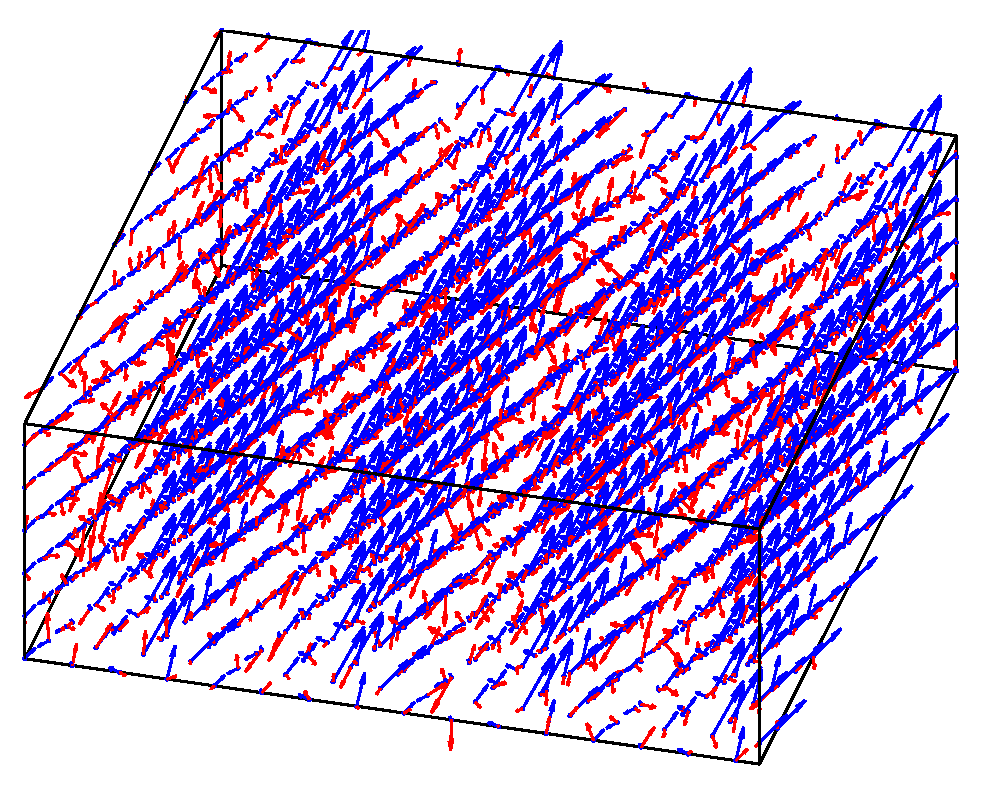
\includegraphics{eigplot.eps}}
\renewcommand{\figure}{Fig.}
\label{fig:bulk_dis_dos}
\end{center}
\end{figure}
\end{columns}
\end{frame}

%%%%%%%%%%%%%%%%%%%%%%%%%%%%%%%%%%%%%%%%%%%%%%%%%%%%%%
%%%%%%%%%%%%%%%%%%%%%%%%%%%%%%%%%%%%%%%%%%%%%%%%%%%%%%
\begin{frame}{Normal Mode Decomposition}
Signal Processing:
Power Spectrum = FFT(XCORR(q))
%%%
%\begin{equation}\label{EQ:NMD:SED}
%\begin{split}
%T\kvw=&\lim_{\tau_0\rightarrow\infty}\frac{1}{2\tau_0}\left|\frac{1}{\sqrt{2\pi}}\int_{0}^{\tau_0}\dot{q}\kvt\exp(-i\omega t)dt\right|^2
%\end{split}
%\end{equation}
%%%
%Expected to have Lorentzian form
%%%
%\begin{equation}\label{EQ:NMD:LOR}
%T\kvw \approx C_0\kv\frac{\Gamma\kv/\pi}{[\omega_0\kv-\omega]^2+\Gamma^2\kv}
%\end{equation}
%%%
%Fitting yields the lifetime
%%%
%\begin{equation}\label{EQ:lifetime}
%\textcolor{blue}{\tau\kv}=\frac{1}{2\Gamma\kv}
%\end{equation}
%%%

\begin{figure}%[H]
\begin{center}
\includegraphics[width=0.4\textwidth]{expplot.eps} \hspace{0.05\textwidth}%
\includegraphics[width=0.4\textwidth]{lorplot.eps} \\[2em]
\end{center}
\end{figure}
\vspace*{-1cm}
Fitting yields the lifetime
%%%
\begin{equation}\label{EQ:lifetime}
\textcolor{blue}{\tau\kv}=\frac{1}{2\Gamma\kv}
\end{equation}
%%%

\end{frame}
%%%%%%%%%%%%%%%%%%%%%%%%%%%%%%%%%%%%%%%%%%%%%%%%%%%%%%
%%%%%%%%%%%%%%%%%%%%%%%%%%%%%%%%%%%%%%%%%%%%%%%%%%%%%%
\begin{frame}{Bulk LJ at 20 K}
\begin{columns}
\column{.3\textwidth}
\begin{table}[h!]
\begin{center}
\begin{tabular*}{\textwidth}{c@{\extracolsep{\fill}}c}
\hline\hline\noalign{\smallskip}
Method & $k$ \\
\noalign{\smallskip}\hline\noalign{\smallskip}
Green-Kubo & 1.2 \\
NMD & 1.2 \\
ALD & 1.3 \\
\hline\hline
\end{tabular*}
\end{center}
\renewcommand{\table}{Table.}
\caption{A comparison of the thermal conductivity prediction methods for bulk LJ argon at 20 K [W/m K].}
\label{TB:K_compare}
\end{table}
\column{.7\textwidth}
\begin{figure}[t]
\begin{center}
\vspace*{-0.8cm}
\scalebox{0.75}{\includegraphics{NMD_v_ALD_bulk.eps}}
\renewcommand{\figure}{Fig.}
\label{fig:nmd_v_ald_bulk}
\end{center}
\end{figure}
\end{columns}
\end{frame}

%%%%%%%%%%%%%%%%%%%%%%%%%%%%%%%%%%%%%%%%%%%%%%%%%%%%%%
%%%%%%%%%%%%%%%%%%%%%%%%%%%%%%%%%%%%%%%%%%%%%%%%%%%%%%
\begin{frame}{Superlattices}
Thermoelectric applications
\begin{itemize}
\item Improve performance the figure of merit by tuning the thermal conductivity
%%%
\begin{equation}\label{EQ:NMD:qdot}
\begin{split}
ZT=\frac{\sigma S^2 T}{k}
\end{split}
\end{equation}
%%%
\item Effect of Period Length
\item Effect of Interfacial Species Mixing
\begin{itemize}
\item \textcolor{orange}{ASSUMPTION}: eigenvectors for perfect SL are valid for mixed SL
\end{itemize}
\end{itemize}
\end{frame}


%%%%%%%%%%%%%%%%%%%%%%%%%%%%%%%%%%%%%%%%%%%%%%%%%%%%%%
%%%%%%%%%%%%%%%%%%%%%%%%%%%%%%%%%%%%%%%%%%%%%%%%%%%%%%
\begin{frame}{\small{4x4 MD Domain}}
\begin{figure}[t]
\begin{center}
\vspace*{-0.8cm}
\scalebox{0.55}{\includegraphics{4p_ai.eps}}
\renewcommand{\figure}{Fig.}
\label{fig:md_domain}
\end{center}
\end{figure}
\end{frame}

%%%%%%%%%%%%%%%%%%%%%%%%%%%%%%%%%%%%%%%%%%%%%%%%%%%%%%
%%%%%%%%%%%%%%%%%%%%%%%%%%%%%%%%%%%%%%%%%%%%%%%%%%%%%%
\section{Results}
\subsection{Dispersion}
\begin{frame}{\small{Dispersion}}
\begin{columns}
\column{.2\textwidth}
Cross-plane (CP)
\newline
\newline
\newline
\newline
\newline
In-plane (IP)
\column{.8\textwidth}
\begin{figure}[!h]
\vspace*{-0.8cm}
\begin{center}
\scalebox{0.48}{ 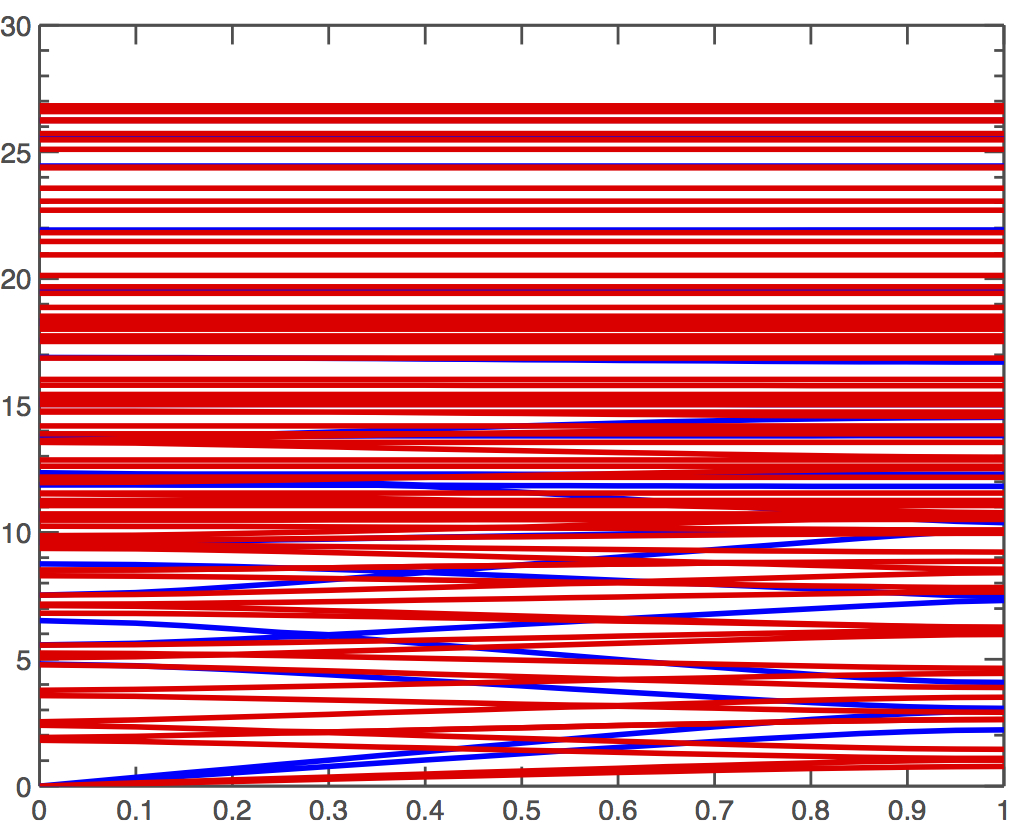
\includegraphics{dispersion.eps}}
\renewcommand{\figure}{Fig.}
\label{fig:sed}
\end{center}
\end{figure}
\begin{figure}[!h]
\vspace*{-0.8cm}
\begin{center}
\scalebox{0.48}{ \includegraphics{dispersion_ip.eps}}
\renewcommand{\figure}{Fig.}
\label{fig:dispersion}
\end{center}
\end{figure}
\end{columns}
\end{frame}


%%%%%%%%%%%%%%%%%%%%%%%%%%%%%%%%%%%%%%%%%%%%%%%%%%%%%%
%%%%%%%%%%%%%%%%%%%%%%%%%%%%%%%%%%%%%%%%%%%%%%%%%%%%%%
\subsection{Power Spectra}
\begin{frame}{Power Spectrum for $4 \times 4$}
\begin{columns}
\column{.075\textwidth}
\begin{figure}[t]
\vspace*{-1cm}
\hspace*{-0.9cm}
%\begin{center}
\includegraphics[height=70mm]{4p_dispersion_only.eps}
\renewcommand{\figure}{Fig.}
\label{fig:disp_4p}
%\end{center}
\end{figure}
\column{.91\textwidth}
\begin{figure}[t]
%\begin{center}
\vspace*{-1.2cm}
\hspace*{1.9cm}
\scalebox{0.60}{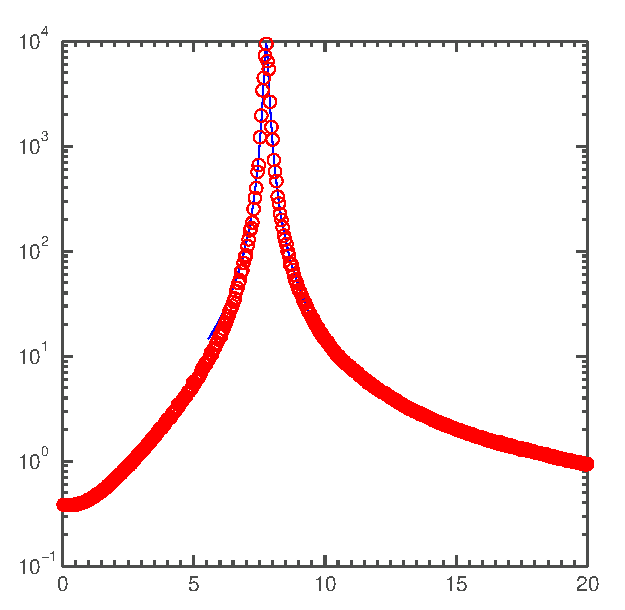
\includegraphics{sed.eps}}
\renewcommand{\figure}{Fig.}
%\caption{(Colour online) Spectral energy density plots for the selected modes along k=[1,0,0] of a 4x4 superlattice as shown in Figure~\ref{fig:dispersion}. Dark blue corresponds to a superlattice without mixing, red corresponds to mixing of 80/20 and light blue corresponds to mixing of 60/40.}
\label{fig:sed}
%\end{center}
\end{figure}
\end{columns}
\end{frame}

%%%%%%%%%%%%%%%%%%%%%%%%%%%%%%%%%%%%%%%%%%%%%%%%%%%%%%
%%%%%%%%%%%%%%%%%%%%%%%%%%%%%%%%%%%%%%%%%%%%%%%%%%%%%%
\subsection{Lifetimes}
\begin{frame}{Lifetimes}
\begin{figure}[!h]
\begin{center}
\vspace*{-0.8cm}
\hspace*{-1cm}
\scalebox{0.65}{\includegraphics{lifvomega_defense.eps}}
\renewcommand{\figure}{Fig.}
\label{fig:lifetimes}
\end{center}
\end{figure}
\end{frame}

%%%%%%%%%%%%%%%%%%%%%%%%%%%%%%%%%%%%%%%%%%%%%%%%%%%%%%
%%%%%%%%%%%%%%%%%%%%%%%%%%%%%%%%%%%%%%%%%%%%%%%%%%%%%%
\subsection{MFP}
\begin{frame}{MFP}
\begin{columns}
\column{.3\textwidth}
$\Lambda \kv=|{\pmb{\mathrm{v}}_{g}\kv}|{\tau\kv}$
\column{.7\textwidth}
\begin{figure}[t]
\begin{center}
\vspace*{-1.5cm}
\scalebox{0.38}{\includegraphics{MFP_cp+ip_cuml_defense.eps}}
\renewcommand{\figure}{Fig.}
\label{fig:mfp_contribution}
\end{center}
\end{figure}
\end{columns}
\end{frame}

%%%%%%%%%%%%%%%%%%%%%%%%%%%%%%%%%%%%%%%%%%%%%%%%%%%%%%
%%%%%%%%%%%%%%%%%%%%%%%%%%%%%%%%%%%%%%%%%%%%%%%%%%%%%%
%\begin{frame}{GK}

%\begin{figure}%[H]
%\begin{center}
%\includegraphics[width=0.3\textwidth]{GK_cp5.eps} \hspace{0.05\textwidth}%
%\includegraphics[width=0.3\textwidth]{/home/schuberm/Dropbox/git/plots.nogit/images/GK_cp7.eps} \\[2em]
%\end{center}
%\end{figure}
%\column{.5\textwidth}
%\begin{figure}%[H]
%\begin{center}
%\includegraphics[width=0.3\textwidth]{/home/schuberm/Dropbox/git/plots.nogit/images/GK_cp8.eps} \hspace{0.05\textwidth}%
%\includegraphics[width=0.3\textwidth]{/home/schuberm/Dropbox/git/plots.nogit/images/GK_cp9.eps} \par
%\end{center}
%\end{figure}

%\end{frame}

%%%%%%%%%%%%%%%%%%%%%%%%%%%%%%%%%%%%%%%%%%%%%%%%%%%%%%
%%%%%%%%%%%%%%%%%%%%%%%%%%%%%%%%%%%%%%%%%%%%%%%%%%%%%%
\subsection{Thermal conductivity}
\begin{frame}{Cross-Plane Perfect SL}
\begin{figure}[t]
\begin{center}
\vspace*{-0.8cm}
\scalebox{0.75}{\includegraphics{KvL_cp.eps}}
\renewcommand{\figure}{Fig.}
\label{fig:cp}
\end{center}
\end{figure}
\end{frame}

%%%%%%%%%%%%%%%%%%%%%%%%%%%%%%%%%%%%%%%%%%%%%%%%%%%%%%
%%%%%%%%%%%%%%%%%%%%%%%%%%%%%%%%%%%%%%%%%%%%%%%%%%%%%%
\begin{frame}{Cross-Plane Mixed SL}
\begin{figure}[t]
\begin{center}
\vspace*{-0.8cm}
\scalebox{0.75}{\includegraphics{KvL_cp_all.eps}}
\renewcommand{\figure}{Fig.}
\label{fig:cp_all}
\end{center}
\end{figure}
\end{frame}

%%%%%%%%%%%%%%%%%%%%%%%%%%%%%%%%%%%%%%%%%%%%%%%%%%%%%%
%%%%%%%%%%%%%%%%%%%%%%%%%%%%%%%%%%%%%%%%%%%%%%%%%%%%%%
\begin{frame}{In-Plane Perfect SL}
\begin{figure}[t]
\begin{center}
\vspace*{-0.8cm}
\scalebox{0.75}{\includegraphics{KvL_ip.eps}}
\renewcommand{\figure}{Fig.}
\label{fig:ip}
\end{center}
\end{figure}
\end{frame}

%%%%%%%%%%%%%%%%%%%%%%%%%%%%%%%%%%%%%%%%%%%%%%%%%%%%%%
%%%%%%%%%%%%%%%%%%%%%%%%%%%%%%%%%%%%%%%%%%%%%%%%%%%%%%
\begin{frame}{In-Plane Mixed SL}
\begin{figure}[t]
\begin{center}
\vspace*{-0.8cm}
\scalebox{0.75}{\includegraphics{KvL_ip_all.eps}}
\renewcommand{\figure}{Fig.}
\label{fig:ip_all}
\end{center}
\end{figure}
\end{frame}

%%%%%%%%%%%%%%%%%%%%%%%%%%%%%%%%%%%%%%%%%%%%%%%%%%%%%%
%%%%%%%%%%%%%%%%%%%%%%%%%%%%%%%%%%%%%%%%%%%%%%%%%%%%%%
\section{Conclusions}
\begin{frame}{Contributions \& Conclusions}
\begin{itemize}
\item Validated GK, DM, ALD, NMD methods for bulk
\item Developed a simple, parallel and open source workflow for NMD
\item First to apply and validate NMD for superlattices
\begin{itemize}
\item Bulk properties are not representative of short-period superlattices
\item Mixing \textit{breaks} secondary periodicity
\end{itemize}
\end{itemize}
\end{frame}

%%%%%%%%%%%%%%%%%%%%%%%%%%%%%%%%%%%%%%%%%%%%%%%%%%%%%%
%%%%%%%%%%%%%%%%%%%%%%%%%%%%%%%%%%%%%%%%%%%%%%%%%%%%%%

\begin{frame}{Acknowledgements}
\begin{itemize}
\item Prof. Cristina Amon
\item Prof. Alan McGaughey
\item Jason Larkin
\item Daniel Sellan
\item Atoms Lab
\item Funding from NSERC, OGS and AMD
\end{itemize}
\end{frame}

%%%%%%%%%%%%%%%%%%%%%%%%%%%%%%%%%%%%%%%%%%%%%%%%%%%%%%
%%%%%%%%%%%%%%%%%%%%%%%%%%%%%%%%%%%%%%%%%%%%%%%%%%%%%%

\begin{frame}{NMD vs. ALD $4 \times 4$ SL}
\begin{figure}[t]
\begin{center}
\vspace*{-0.8cm}
\scalebox{0.75}{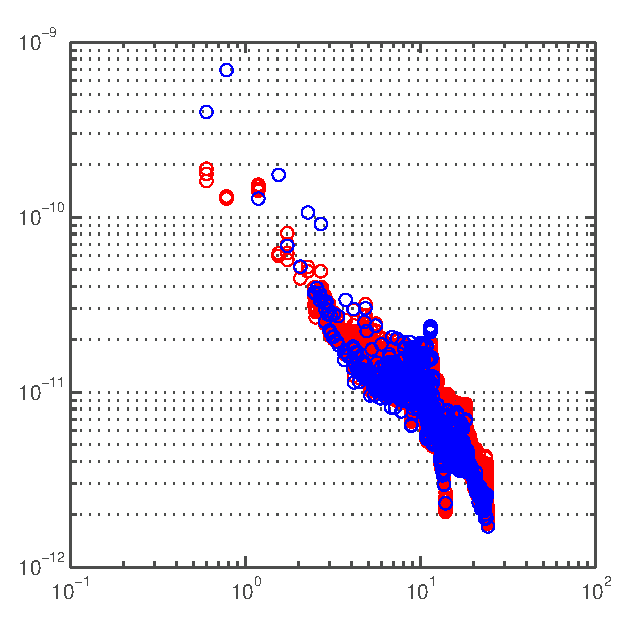
\includegraphics{NMD_v_ALD.eps}}
\renewcommand{\figure}{Fig.}
\label{fig:NMD_v_ALD_sl}
\end{center}
\end{figure}
\end{frame}

%%%%%%%%%%%%%%%%%%%%%%%%%%%%%%%%%%%%%%%%%%%%%%%%%%%%%%
%%%%%%%%%%%%%%%%%%%%%%%%%%%%%%%%%%%%%%%%%%%%%%%%%%%%%%

\begin{frame}{Green-Kubo}
\begin{figure}[t]
\begin{center}
\vspace*{-0.8cm}
\scalebox{0.75}{\includegraphics{GK_bulk.eps}}
\renewcommand{\figure}{Fig.}
\label{fig:GK_bulk}
\end{center}
\end{figure}
\end{frame}


%%%%%%%%%%%%%%%%%%%%%%%%%%%%%%%%%%%%%%%%%%%%%%%%%%%%%%
%%%%%%%%%%%%%%%%%%%%%%%%%%%%%%%%%%%%%%%%%%%%%%%%%%%%%%

\begin{frame}{Size effects}
\begin{table}
\begin{tabular*}{\textwidth}{c@{\extracolsep{\fill}}ccccc}
\hline\hline\noalign{\smallskip}
Cross-Plane& \multicolumn{4}{c}{$N\times N$ Superlattice} \\
\cline{2-5}\noalign{\smallskip}
$N_xN_yN_z$ & $2\times2$ & $4\times4$ & $8\times8$ & $14\times14$  \\
\noalign{\smallskip}\hline\noalign{\smallskip}
$4\times6\times6$ & 0.15  & 0.17  &  0.15  &  0.21 \\
$6\times6\times6$ & 0.23  & 0.22  &  0.28  &  0.36 \\
$8\times6\times6$ & 0.28  & 0.23  &  0.32  &  0.39 \\
$10\times6\times6$ & 0.29  &   &    &   \\
\hline\hline
\label{TB:K_CP_NMDsize}
\end{tabular*}
\renewcommand{\table}{Table.}
\caption{A comparison of the CP thermal conductivity NMD predictions [W/m K].}
\end{table}
\end{frame}

%%%%%%%%%%%%%%%%%%%%%%%%%%%%%%%%%%%%%%%%%%%%%%%%%%%%%%
%%%%%%%%%%%%%%%%%%%%%%%%%%%%%%%%%%%%%%%%%%%%%%%%%%%%%%

\begin{frame}{Size effects}
\begin{table}
\begin{tabular*}{\textwidth}{c@{\extracolsep{\fill}}ccccc}
\hline\hline\noalign{\smallskip}
In-Plane& \multicolumn{4}{c}{$N\times N$ Superlattice} \\
\cline{2-5}\noalign{\smallskip}
$N_xN_yN_z$ & $2\times2$ & $4\times4$ & $8\times8$ & $14\times14$  \\
\noalign{\smallskip}\hline\noalign{\smallskip}
$4\times6\times6$ & 0.53 & 0.52  &  0.56  &  0.69 \\
$6\times6\times6$ & 0.53 & 0.51  &  0.56  &  0.59 \\
$8\times6\times6$ & 0.52 & 0.51  &  0.55  &  0.58 \\
\hline\hline
\end{tabular*}
\renewcommand{\table}{Table.}
\caption{A comparison of the IP thermal conductivity NMD predictions [W/m K].}
\label{TB:K_IP_NMDsize}
\end{table}
\end{frame}

%%%%%%%%%%%%%%%%%%%%%%%%%%%%%%%%%%%%%%%%%%%%%%%%%%%%%%
%%%%%%%%%%%%%%%%%%%%%%%%%%%%%%%%%%%%%%%%%%%%%%%%%%%%%%
\subsection{MFP}
\begin{frame}{MFP}
\begin{figure}[t]
\begin{center}
\vspace*{-0.8cm}
\scalebox{0.55}{\includegraphics{MFP_cp_defense.eps}}
\renewcommand{\figure}{Fig.}
\label{fig:mfp_contribution}
\end{center}
\end{figure}
\end{frame}

%%%%%%%%%%%%%%%%%%%%%%%%%%%%%%%%%%%%%%%%%%%%%%%%%%%%%%
%%%%%%%%%%%%%%%%%%%%%%%%%%%%%%%%%%%%%%%%%%%%%%%%%%%%%%

\begin{frame}{MD Configurations}
\begin{table}
\begin{tabular*}{\textwidth}{c@{\extracolsep{\fill}}ccccc}
\hline\hline\noalign{\smallskip}
&\multicolumn{4}{c}{Superlattice} \\
\cline{2-5}\noalign{\smallskip}
\hspace{1cm} & $2\times2$ & $4\times4$ & $8\times8$ & $14\times14$  \\
\noalign{\smallskip}\hline\noalign{\smallskip}
FFT window, $\tau_0$  & $2^{16}/2^{16}$ & $2^{16}/2^{16}$ & $2^{16}$/$2^{20}$ &$ 2^{16}$/$2^{22}$\\
Total MD timesteps & $2^{20}/2^{20}$ &  $2^{20}/2^{20}$ & $2^{20}$/$2^{20}$  & $2^{20}$/$2^{22}$\\
Number of Seeds & 5/5 &  5/5 & 5/10  &  5/10\\
\hline\hline
\end{tabular*}
\renewcommand{\table}{Table.}
\caption{Number of timesteps in the Fourier sampling windows ($\omega_H \kv \geq 1$/$\omega_H \kv < 1$), total number of MD timesteps for each superlattice system, and the total number of independent MD simulations. The use of $\omega_H\kv=1$ as the transition frequency was found to be suitable in order to obtain convergence for lifetime estimate and satisfy the $\Gamma\kv \ll \omega_H\kv$ condition.}
\label{TB:MD_time}
\end{table}

\begin{itemize}
\item The MD simulations time step is 4.285 fs (0.002 in LJ units). Equilibration is achieved by running a NVE ensemble with velocity rescaling for $1\times 10^5$ timesteps followed by a NVE ensemble for $2.5 \times10^5$ timesteps
\end{itemize}
\end{frame}

%%%%%%%%%%%%%%%%%%%%%%%%%%%%%%%%%%%%%%%%%%%%%%%%%%%%%%
%%%%%%%%%%%%%%%%%%%%%%%%%%%%%%%%%%%%%%%%%%%%%%%%%%%%%%

\begin{frame}{Experimental Measurements}
\begin{figure}[t]
\begin{center}
\vspace*{-0.8cm}
\scalebox{0.3}{\includegraphics{experiment.jpeg}}
\renewcommand{\figure}{Fig.}
\label{fig:GK_bulk}
\caption{Diagram of Frequency Domain Thermoreflectance set-up. Courtesy: Regner et al. 2013 Nature Communications}
\end{center}
\end{figure}
\end{frame}

\end{document}
